\chapter{Asking Millionaires How They Got Rich: Silicon Valley}

These notes follow a School of Hard Knocks field interview, curated by LazyingArt LLC. There are no validated equation-bearing frames for this lecture, so the mathematics is necessarily transcript-level: a few hard numbers, a few careful compressions, and a strong insistence that we keep the order of discovery intact. The lecture itself unfolds as a search. First we see wealth. Then we discover how hard it is to make wealth speak. Only after that do the governing mechanisms become clear.

\section{Wealth Before Explanation}

We begin, as the lecture begins, with outcomes rather than doctrine. The cold open throws four cases at us in rapid sequence: a Ferrari, a founder who sold a company for a little north of \(70\) million dollars, a satellite entrepreneur who won a government contract worth billions, and a plastic surgeon whose route to wealth ran through practice rather than through software or venture finance. The point is not yet to explain anything. The point is to establish scale.

The opening line about having ``grown it to \(17\) million dollars'' is almost certainly a garbled transcript. Later repetitions stabilize the claim: the host grew a channel to \(17\) million followers. We should keep that correction in mind, because the follower count becomes part of the lecture's method. It is one of the few pieces of leverage the host has when trying to interrupt rich people in motion.

This opening sequence matters structurally. The lecture does not begin with a thesis about Silicon Valley; it begins with a payoff reel. Only after we have seen the range of possible outcomes does the lecture reset and tell us where we are.

\section{Silicon Valley as a Wealth Field, and the Difficulty of Access}

The formal introduction now arrives. Silicon Valley is described as the place that created more billionaires than anywhere else on Earth, the home of giant companies, bold ideas, and concentrated innovation. But the lecture immediately introduces a second fact that is at least as important: visible wealth is not the same thing as usable access.

The host's own scale markers are part of the setup:
\begin{align}
F_{\text{host}} &= 17 \times 10^6,\\
N_{\text{billionaires interviewed}} &= 25,\\
N_{\text{billionaires,SV}} &\approx 75.
\end{align}
These are not deep equations, but they explain why the host expects the trip to yield doctrine. If one has interviewed \(25\) billionaires and built an audience of \(17\) million, one might think proximity can be converted into instruction. The refusal montage shows otherwise.

Repeatedly, the answer is no: no press, no video, no time, no interview. What the lecture teaches here is not merely social awkwardness. It teaches that a rich field can still have a severe information bottleneck. The difficulty of the early minutes is part of the argument.

We can therefore summarize the access logic as
\begin{equation}
\text{visible wealth}
\;\to\;
\text{cold approach}
\;\to\;
\text{refusal}
\;\to\;
\text{credibility proof}
\;\to\;
\text{partial answer}.
\end{equation}
This is not a speaker-stated formula. It is an editorial compression of the lecture's first movement.

\subsection{Question \& Answer}

\paragraph{Question.} If the money is visibly everywhere, why is usable advice still so hard to obtain?

\paragraph{Answer.} Because the scarce variable is not wealth but attention. The lecture makes this point theatrically. The rich people are present, but they are moving, private, and not automatically interested in turning their lives into public instruction. The host must spend his own credibility simply to buy a few minutes. In that sense, the lecture begins with an access constraint before it reaches any business principle.

\begin{figure}[h]
\centering
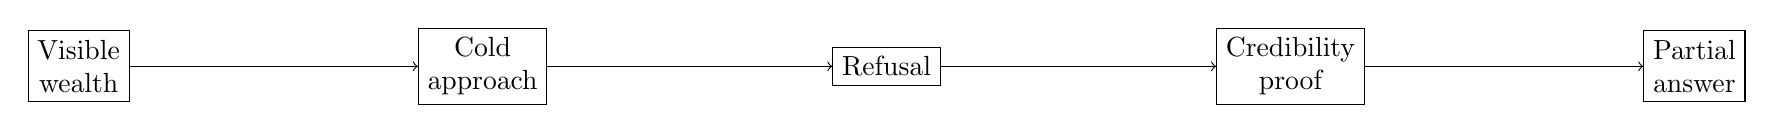
\begin{tikzpicture}[x=2.7cm,y=1.25cm]
\node[draw, align=center] (a) at (0,0) {Visible\\wealth};
\node[draw, align=center] (b) at (1.9,0) {Cold\\approach};
\node[draw, align=center] (c) at (3.8,0) {Refusal};
\node[draw, align=center] (d) at (5.7,0) {Credibility\\proof};
\node[draw, align=center] (e) at (7.6,0) {Partial\\answer};
\draw[->] (a) -- (b);
\draw[->] (b) -- (c);
\draw[->] (c) -- (d);
\draw[->] (d) -- (e);
\end{tikzpicture}
\caption{A transcript-derived access funnel. In this lecture, advice is extracted under pressure rather than delivered in seminar form.}
\end{figure}

The host's own recap after the refusals is important. He tells us that these people are private and that he will keep pushing until he can extract ``a billion dollars worth of gain.'' That recap is the hinge. It turns failure into method and prepares the way for the first short success.

\section{A One-Minute Venture-Capital Doctrine}

The first successful encounter is a venture capitalist, and the lecture makes good use of the time pressure. The answers are compressed, sometimes almost reluctant, but that is precisely why they matter. We are not receiving a full theory of venture finance. We are receiving what survives severe compression.

The first criterion is market opportunity. A cautious formalization is
\begin{equation}
P(\text{funding}) \uparrow
\qquad \text{as} \qquad
M_{\text{opp}} \uparrow,
\end{equation}
where \(M_{\text{opp}}\) is perceived market opportunity. That is the VC's first answer, and it should remain the first principle in our notes.

The second theme is AI. The VC says that anything to do with AI is a major opportunity and agrees that firms ignoring AI risk being left behind. The lecture offers no deeper derivation than this, but the point is clear enough: AI is being treated as a general multiplier on reachable value.

The third theme is even more basic, and more durable:
\begin{equation}
N_{\text{customers}} = 0
\qquad \Longrightarrow \qquad
\text{business} = 0.
\end{equation}
The most memorable sentence in the exchange is not about valuation or prestige. It is about customers. The customer comes first because without customer purchase there is no business to optimize.

Finally, when the host asks how one raises money in the competitive world of venture capital itself, the answer becomes track record. We might say: promise attracts attention, but proof attracts capital.

\subsection{Question \& Answer}

\paragraph{Question.} What is the minimum credible signal that makes a founder or a fund manager worth backing?

\paragraph{Answer.} In the lecture's compressed form, the signal is not eloquence. It is a conjunction of three things: a large market opportunity, genuine contact with customer demand, and a demonstrated record of making money for other people. The host's own recap reduces the interview still further: use AI, and put the customer first.

This recap matters. The host does not pretend he received a full interview. He tells us what he actually extracted. That habit of extraction and recap is part of the lecture's rhythm, and we should preserve it on the page.

\section{The \(70\)-Million-Dollar Exit That Revenue Cannot Explain}

Now the lecture slows down. This is its main analytic center. A founder says he became rich young by building a point-of-sale device and selling the company for a little north of \(70\) million dollars. Then he provides the cluster of numbers that gives the story its force:
\begin{align}
V_{\text{exit}} &\gtrsim 70 \times 10^6 \ \text{dollars},\\
R &\approx 60 \times 10^3 \ \text{dollars},\\
C &\approx 17 \times 10^6 \ \text{dollars}.
\end{align}
Here \(R\) is reported revenue and \(C\) is the speaker's cumulative spend on the company. These are spoken quantities, not audited statements, but they are the lecture's clearest numerical payload.

If we reason only from seller-side revenue, the exit looks absurd. That is exactly the point. The lecture wants to break the reflex that says present revenue must be the main explanatory variable.

\paragraph{Worked derivation.} The contrast ratios make the point sharply:
\begin{align}
\frac{V_{\text{exit}}}{R}
&\approx
\frac{70 \times 10^6}{60 \times 10^3}
\approx 1.17 \times 10^3,\\
\frac{C}{R}
&\approx
\frac{17 \times 10^6}{60 \times 10^3}
\approx 2.83 \times 10^2.
\end{align}
So the company had both tiny revenue relative to the exit and huge spend relative to revenue. We should not try to domesticate this into a comfortable compounding story. The founder is explicitly telling us that the deal cannot be understood on ordinary trailing-revenue terms.

The explanation is buyer-side value. The founder says the buyer already had roughly
\begin{equation}
N_{\text{sales}} \approx 11{,}000
\end{equation}
sales representatives, and that the process of scaling by another
\begin{equation}
\Delta N_{\text{sales}} \approx 9{,}000
\end{equation}
would itself have been worth on the order of
\begin{equation}
V_{\text{buyer-side}} \approx 70\text{--}80 \times 10^6 \ \text{dollars}.
\end{equation}
In other words, the sale price is being anchored to avoided buyer friction, not to seller revenue.

\begin{definition}
We will call
\begin{equation}
V_{\text{buyer-side}}
\approx
V_{\text{fit}} + V_{\text{function}} + V_{\text{avoided friction}}
\end{equation}
the buyer-side value of the acquisition.
\end{definition}

\begin{remark}
This is a cautious reconstruction of the founder's logic, not a board equation from a visible frame. But it is the cleanest way to formalize what he means by ``fit and function'' and by the claim that price is only an issue if value is absent.
\end{remark}

\subsection{Question \& Answer}

\paragraph{Question.} How can a company with tiny revenue command a large exit?

\paragraph{Answer.} Because revenue is not the only thing being priced. In this story, the relevant quantity is what the buyer saves in delay, coordination, hiring, and deployment. A concise statement of the lecture's logic is
\begin{equation}
V_{\text{exit}} \approx V_{\text{buyer-side}}.
\end{equation}
The founder's further remark, ``value is only in the eye of the beholder,'' makes the same point from the other side. He is not claiming that accounting numbers do not matter. He is claiming that, in acquisition, the buyer's problem can dominate the seller's current income statement.

\begin{figure}[h]
\centering
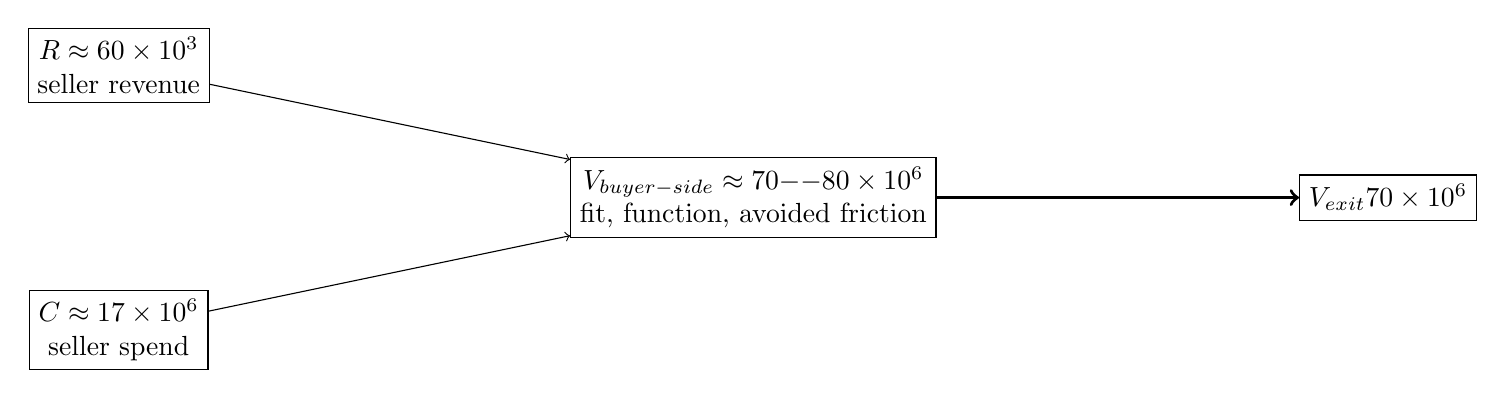
\begin{tikzpicture}[x=3.1cm,y=1.4cm]
\node[draw, align=center] (r) at (0,1.2) {$R \approx 60 \times 10^3$\\seller revenue};
\node[draw, align=center] (c) at (0,-1.2) {$C \approx 17 \times 10^6$\\seller spend};
\node[draw, align=center] (b) at (2.6,0) {$V_{\text{buyer-side}} \approx 70\text{--}80 \times 10^6$\\fit, function, avoided friction};
\node[draw, align=center] (e) at (5.2,0) {$V_{\text{exit}} \gtrsim 70 \times 10^6$};
\draw[->] (r) -- (b);
\draw[->] (c) -- (b);
\draw[->, very thick] (b) -- (e);
\end{tikzpicture}
\caption{A transcript-derived reading of the point-of-sale exit. The surprising quantity is not seller revenue but buyer-side savings.}
\end{figure}

The lecture is not finished with this speaker. Having established one striking deal, it now enlarges the witness. He says he later built and sold five more companies, including one sale to Facebook, one to NetSuite/Oracle, and another exit around \(285\) million dollars. The move is important: the chapter's central witness is no longer merely a lucky founder with one strange transaction. He is being presented as someone with repeated commercial pattern recognition.

\section{Switchgear, Capacity Shortage, and the Wealth of Bottlenecks}

The lecture now pivots, through the same founder, from exits into biography and industry selection. He says he did not learn to read until the ninth grade, had no parents, and effectively taught himself into entrepreneurship. His high-school senior project became a business, and a grandmother's \(70{,}000\)-dollar check helped launch the first real effort. We should keep this widening of frame. The lecture is no longer speaking only through arithmetic; it is tying arithmetic to a life.

When asked what industry matters now, the answer is not glamorous software. It is energy, infrastructure, and manufacturing, especially switchgear. This is one of the lecture's most useful corrections. The host comes to Silicon Valley seeking future-tech doctrine; the founder replies with an old industrial choke point.

The strongest numerical claim is about capacity. A study attributed to Amazon is paraphrased as follows: even if Amazon absorbed all U.S. switchgear manufacturing capacity for the next ten years, it would still satisfy only about \(25\%\) of what it needed. We may write this as
\begin{equation}
\frac{K_{\text{available}}}{D_{\text{Amazon need}}} \approx 0.25.
\end{equation}
Rearranging gives the implied demand gap:
\begin{equation}
D_{\text{Amazon need}} \approx 4 K_{\text{available}}.
\end{equation}
This is the heart of the segment. The opportunity is not that switchgear is fashionable. It is that shortage is structural.

The founder then reports the economics of his own position:
\begin{align}
K_{\text{rev}} &\approx 1.2 \times 10^9 \ \text{dollars},\\
\rho_g &\approx 0.5.
\end{align}
The implied gross-profit capacity is therefore
\begin{equation}
\Pi_g \approx \rho_g K_{\text{rev}}
\approx 0.5 \times 1.2 \times 10^9
\approx 0.6 \times 10^9 \ \text{dollars}.
\end{equation}
This is why the phrase ``software money out of manufacturing'' is more than a slogan. It is a compressed numerical judgment about what scarcity can do to margin.

The ticket sizes make the scale vivid:
\begin{align}
P_{\text{building switchgear}} &\approx 15 \times 10^6 \ \text{dollars},\\
P_{\text{small data center}} &\approx 15\text{--}20 \times 10^6 \ \text{dollars},\\
P_{\text{large data center}} &\approx 1 \times 10^9 \ \text{dollars}.
\end{align}
We should notice the logic here. The lecture is not saying that any old product is a fortune. It is saying that a dull product sitting at an infrastructural bottleneck can become extremely lucrative.

\subsection{Question \& Answer}

\paragraph{Question.} Why can an old industrial product generate software-like money?

\paragraph{Answer.} Because ``old'' does not mean ``commoditized'' when demand is exploding and capacity is scarce. The switchgear story combines replacement demand, new data-center demand, very large ticket sizes, and insufficient supply. Under those conditions the business inherits some of the economic features we usually associate with software: selective customers, pricing power, and unusually large margins.

The founder also mentions a current growth ladder,
\begin{equation}
5 \times 10^6 \to 50 \times 10^6 \to 300 \times 10^6,
\end{equation}
not as audited history but as a way of conveying how quickly scale can shift once the industry choice is right.

Then the lecture widens once more. The same founder, having spoken about acquisition logic and switchgear margins, turns to the Bible, to Christian apologetics, and to a design-creator argument. One may agree or disagree, but the formal point is important: the lecture refuses to leave the human being behind after extracting the arithmetic. The same witness who reasons about capacity also reasons about meaning.

\paragraph{Structural interruption.} At this point the lecture breaks into a long promotional appeal for a mentorship community. The content is heavily promotional and often garbled in the transcript. Still, it should not be dropped completely, because it explains something real about the lecture's structure: hard-won proximity is being converted into a commercial promise of mediated access.

\section{After the Interruption: Apple and Satellites}

The lecture returns from the interruption by broadening its taxonomy of wealth. We are no longer in a single-founder world. Instead, we get two alternative routes: adjacency to a great company, and repair of a broken one.

\paragraph{Apple: wealth by long-duration exposure.} The Ferrari owner in the resumed segment did not become rich by founding Apple. He worked there, rose to engineering director, stayed for almost two decades, and says plainly that the wealth vehicle was Apple stock. The clean editorial compression is
\begin{equation}
W_{\text{employee}} \approx Y_{\text{salary}} + G_{\text{stock}},
\end{equation}
with the second term carrying the asymmetry.

The tenure number is explicit:
\begin{equation}
t_{\text{Apple}} \approx 20 \ \text{years}.
\end{equation}
The lecture's point is not merely ``right place, right time.'' It is that corporate employment can still be a serious wealth path when one attaches early and for a long time to an exceptional firm. The speaker's further remarks sharpen the contrast with the VC segment: he is skeptical of crowded AI enthusiasm, prefers a contrarian posture, and reduces the Apple lesson to one sentence, ``set a high bar.''

\paragraph{Satellites: wealth by fixing the broken system.} The next speaker says he became a millionaire later, perhaps around fifty, by building a satellite company. The origin story is precise in spirit even if not in accounting detail. After \(9/11\), he found a company that was broken and believed the world needed more information about itself.

The scale marker is coarse but unmistakable: one U.S. government contract was on a multi-billion-dollar scale. The work pattern is more precise:
\begin{equation}
T_{\text{work}} \in \{6,7\} \ \text{days per week}.
\end{equation}
The lecture pairs that with sacrifice: missed family events, years of intense work, and the claim that the result made the country safer, protected the environment, created jobs, and enriched investors.

\subsection{Question \& Answer}

\paragraph{Question.} What makes a broken business worth fixing rather than abandoning?

\paragraph{Answer.} In the lecture's answer, a broken business is one whose offer no longer matches the real need. The satellite founder states the rule directly: businesses go wrong when they sell what they have, not what the customer needs. A cautious formalization is
\begin{equation}
\text{commercial fit} \uparrow
\qquad \text{as} \qquad
\|\text{offer} - \text{customer need}\| \downarrow.
\end{equation}
In this case the unmet need was information: digital maps, geographic knowledge, and situational visibility at a time when such tools were not yet taken for granted.

This is why the lecture does not reduce the outcome to luck. Luck matters; the speaker says so. But the commercial mechanism is still legible. The company aligned its offer with a need that was becoming urgent. The same speaker then makes a further forecast: cyber will matter more because AI makes deception easier. That is an elegant late echo of the earlier VC segment. AI first appeared there as opportunity; here it returns as attack surface.

\section{Plastic Surgery and the Economics of Happiness}

The closing case broadens the lecture one last time. The speaker is a plastic surgeon, a farm boy from Illinois with what he calls a misspent youth, who worked hard and made his patients happy. The lecture does not treat this as a novelty act. It treats it as a legitimate wealth mechanism in the same field as venture, acquisitions, and industrial bottlenecks.

The most concrete numerical anchor is a procedure ticket:
\begin{equation}
P_{\text{surgery}} \approx 20{,}000 \ \text{dollars}.
\end{equation}
Patients, he says, bring that kind of cash for surgery, and they are not necessarily elites. Some are ordinary people who own businesses and worked hard. The point is not only willingness to pay. The point is that a high ticket can coexist with perceived benefit.

The surgeon's own account is strikingly simple. He wanted to make people happy. He chose the field because he enjoyed it. Technology improved the results, improved healing, and made patients happier still. In this final movement, the lecture becomes almost classical: skill, satisfaction, and reputation reinforce one another.

\subsection{Question \& Answer}

\paragraph{Question.} Can making people happier be a real business model rather than a sentimental slogan?

\paragraph{Answer.} The lecture's answer is yes, provided the happiness is attached to real competence and real outcome. The surgeon does not deny that money is made. He says instead that happiness may matter more than money. A cautious compression of the commercial logic is
\begin{equation}
\text{service strength} \uparrow
\qquad \text{as} \qquad
\text{client happiness} \uparrow.
\end{equation}
This is a softer relation than the switchgear margin formula, but it is not empty. It says that in a service business, satisfaction is not decorative. It is one of the things being sold.

The lecture therefore ends in the right place. After Ferrari shots, billion-dollar contracts, and venture-capital formulas, we close on a field in which business success can still be tied to making other people better off.

\section{Summary}

What begins as spectacle turns, step by step, into discrimination. Silicon Valley is first presented as a dense wealth field, then as a field with severe access friction, and only then as a collection of distinct commercial mechanisms. A venture capitalist emphasizes market opportunity, AI, customer primacy, and track record. A founder explains how a company with almost no revenue can sell for tens of millions when buyer-side savings dominate seller-side accounting. The same founder then moves from software exits to switchgear, showing that scarcity at an industrial bottleneck can produce software-like economics. After a structural interruption, the lecture adds two more routes: long-term stock exposure inside Apple, and the repair of a broken satellite company by selling what customers actually need. Finally, the plastic-surgery case reminds us that service quality and human happiness can themselves be commercial variables.

The chapter's governing lesson is therefore not that Silicon Valley is rich. It is that wealth is made by structure: by market size, by bottleneck position, by buyer-side value, by stock exposure, by institutional need, or by service quality. If we keep that order of discovery, the lecture reads not as hype but as a field report on commercial mechanism.